\section{Mapeamento}

\section{Tipos de Restrições}

O produto da compilação realizada pelo Satyrus é uma equação de energia da forma
\begin{equation}
    E\left({\vec{x}}\right) = E_{0}\left({\vec{x}}\right) + \sum_{i} \lambda_{i}\, E_{i}\left({\vec{x}}\right) \label{eq:energy}
\end{equation}
Onde $E_0 (\vec{x})$ representa o custo imposto pelas restrições de otimalidade e $E_i \left(\vec{x}\right)$ aquele oriundo das restrições de integridade. Os pesos $\lambda_{i}$ dizem respeito às penalidades aplicadas sobre cada nível $i$ da hierarquia de restrições. Trataremos com cuidado das suas especificidades em breve.

A geração de $E\left(\vec{x}\right)$ supõe resolver um problema de programação inteira onde as entradas de $\vec{x}$ assumem valores binários e deseja-se minimizar o valor de $E(\vec{x})$.
\begin{align}
     & \min E(\vec{x})                            \\
     & \text{t.q.}~\vec{x} \in \mathbb{B}^{n} \nonumber
\end{align}


\subsection{Restrições de Otimalidade} \label{subsec:opt-cons}

\subsection{Restrições de Integridade} \label{subsec:int-cons}








\section{Cálculo das Penalidades}

Cada penalidade $\lambda_{i}$ é construída de maneira que a violação de qualquer cláusula pertencente ao $i$-ésimo nível induza à energia total um valor maior do que aquele gerado pela violação de todas as cláusulas presentes nos níveis inferiores. De maneira um pouco mais abstrata, é preciso que a penalidade $\lambda_{i}$, somada ao custo da configuração de menor valor dos níveis anteriores, seja maior do que a mais alta energia que estes possam proporcionar.

Tendo isso em mente, definimos
\begin{equation}
    \left. E \left({ \vec{x} }\right)\right|_{i} = E_0 \left({ \vec{x} }\right) + \sum_{j < i} \lambda_{j}\, E_{j} \left({ \vec{x} }\right) \nonumber
\end{equation}
como sendo a equação de energia correspondente aos níveis de penalidade inferiores a $i$. Seu custo é idêntico àquele obtido por $E\left({\vec{x}}\right)$ em estados que não violam restrições do nível $i$ em diante.

Assim, dizemos ser necessário que
\begin{equation}
    \lambda_{i} > \max \left. E \left({ \vec{x} }\right)\right|_{i} - \min \left. E \left({ \vec{x} }\right)\right|_{i} \label{eq:penalty-bounds}
\end{equation}
Aqui lembramos que cada $E_j : \mathbb{B}^{n} \to \mathbb{N}$ com $j > 0$ conta o número $n_j$ de cláusulas violadas no nível $j$. Portanto, para as funções relativas às restrições de integridade, temos $\max E_j \left({ \vec{x} }\right) = n_j$ e $\min E_j \left({ \vec{x} }\right) = 0$. Isso nos permite reescrever \eqref{eq:penalty-bounds} como
\begin{equation}
    \lambda_{i} > \mu_0 + \sum_{j < i} \lambda_{j}\, n_j \label{eq:penalty-ineq}
\end{equation}
onde $\mu_0 = \max E_0 \left({ \vec{x} }\right) - \min E_0 \left({ \vec{x} }\right)$.

Tomando a diferença entre as penalidades de níveis consecutivos é possível obter uma expressão para calcular cada $\lambda_{i}$ eficientemente através de um processo iterativo. A partir de \eqref{eq:penalty-ineq} fazemos
\begin{equation}
    \lambda_{i + 1} - \lambda_{i} > \left({\mu_0 + \sum_{j \le i} \lambda_{j}\, n_j}\right) - \left({\mu_0 + \sum_{j < i} \lambda_{j}\, n_j}\right) = \lambda_{i}\,n_{i} \nonumber
\end{equation}
ou seja,
\begin{equation}
    \lambda_{i + 1} > \lambda_{i}\, (n_{i} + 1) \nonumber
\end{equation}

Escolhendo $\varepsilon > 0$ arbitrariamente pequeno, escrevemos
\begin{equation}
    \lambda_{i + 1} = \lambda_{i}\, (n_{i} + 1) + \varepsilon
\end{equation}

Ainda nos resta calcular $\mu_0$. Conhecer máximo e mínimo de $E_0 \left({\vec{x}}\right)$, a princípio, é simplesmente o caso irrestrito do próprio problema que desejamos resolver. Sabendo, contudo, que $E_{i} \left({\vec{x}}\right)$ é da forma
\begin{equation}
    E_{i} \left({\vec{x}}\right) = \sum_{\omega \in \Omega_{i}} c_{\omega} \prod_{k \in \omega} \vec{x}_{k}
\end{equation}
podemos obter cotas inferiores e superiores através de seus coeficientes $c_\omega$. Para a cota inferior, somaremos todos os valores negativos, uma vez que é sempre possível escolher $\vec{x} = 0$ para obter tal limite. Para a cota superior, consideramos os valores estritamente positivos. Em ambos os casos, não poderíamos esquecer de adicionar eventuais termos constantes, isto é, $c_\omega$ quando $\omega = \varnothing$. Como tomaremos imediatamente a diferença entre as cotas, isso não será relevante. Concluindo,
\begin{align}
    \mu_0 &= \sum_{\omega \in \Omega_0} \frac{c_\omega + \left|c_\omega\right|}{2} - \sum_{\omega \in \Omega_0} \frac{c_\omega - \left|c_\omega\right|}{2} \nonumber \\
    &= \sum_{\omega \in \Omega_0} \left|c_\omega\right|
\end{align}

\section{SATish}

\section{WTA}

%%\input{figures/compiler-wta.tex}

%%\begin{figure}[H]
    %%
    %
    \def\w{3.2cm}
    \def\s{0.3cm}
    \def\h{1.0cm}

    \def\stack#1#2#3{\node[rectangle] (input) at (\w * #1 + \s * #1, \h * #2) {#3};}
    \def\xtack#1#2#3{\node[rectangle, fill=none, draw=none] (input) at (\w * #1 + \s * #1, \h * #2) {};}
    \def\arrow#1{\draw[->] (\w * #1 + \s * #1 + \w * 0.5, 0) -- (\w * #1 + \s * #1 + \w * 0.5 + \s, 0);}
    \def\base#1#2{\node[rectangle, fill=#2!30, minimum height=0.2cm] (input) at (\w * #1 + \s * #1, -\h+0.25cm) {};}
    %
    %%
    \centering
    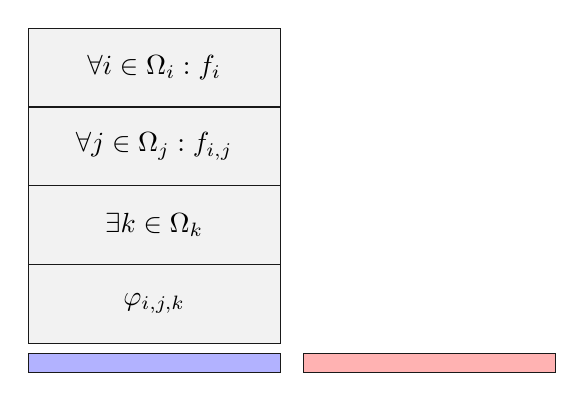
\begin{tikzpicture}[nodes={draw=black!90, fill=gray!10,
        minimum height=\h,
        minimum width=\w,
        },
    row sep=0.3cm,column sep=0.5cm]
        \base{0}{blue}
        \stack{0}{3}{$\forall i\in \Omega_i : f_i$}
        \stack{0}{2}{$\forall j \in \Omega_j : f_{i, j}$}
        \stack{0}{1}{$\exists k \in \Omega_k$}
        \stack{0}{0}{$\varphi_{i, j, k}$}
        %\arrow{0}
        \base{1}{red}
        %\stack{1}{3}{$\forall i\in \Omega_i$}
        %\stack{1}{2}{$\forall j \in \Omega_j$}
        %\stack{1}{1}{$\exists k \in \Omega_k$}
        %\stack{1}{0}{$\Phi_{i, j, k}$}
        %\arrow{1}
    \end{tikzpicture}
    \bigskip\break
    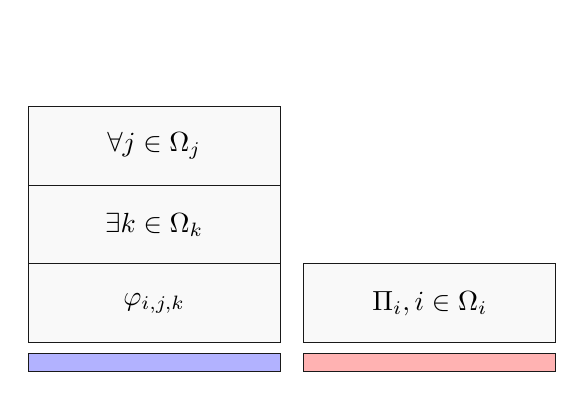
\begin{tikzpicture}[nodes={draw=black!90, fill=gray!5,
        minimum height=\h,
        minimum width=\w,
        },
    row sep=0.3cm,column sep=0.5cm]
        \base{0}{blue}
        \xtack{0}{3}{$\forall i\in \Omega_i$}
        \stack{0}{2}{$\forall j \in \Omega_j$}
        \stack{0}{1}{$\exists k \in \Omega_k$}
        \stack{0}{0}{$\varphi_{i, j, k}$}
        %\arrow{0}
        \base{1}{red}
        \stack{1}{0}{$\Pi_{i}, i\in \Omega_i$}
        %\stack{1}{2}{$\forall j \in \Omega_j$}
        %\stack{1}{1}{$\exists k \in \Omega_k$}
        %\stack{1}{0}{$\Phi_{i, j, k}$}
        %\arrow{1}
    \end{tikzpicture}
    %%
    \label{fig:compiler-stack}
    \caption{O processo de análise dos quantificadores.}
\end{figure}